\documentclass[aspectratio=169]{beamer}
\mode<presentation>
{
  \usetheme{metropolis}      % or try Darmstadt, Madrid, Warsaw, ...
  \usecolortheme{default} % or try albatross, beaver, crane, ...
  \usefonttheme{structurebold}  % or try serif, structurebold, ...
  \setbeamercolor{background canvas}{bg=white}
  \setbeamertemplate{navigation symbols}{}
  \setbeamertemplate{bibliography item}{\insertbiblabel}
  %\setbeamertemplate{caption}[numbered]
} 
\usepackage[english]{babel}
\usepackage[utf8x]{inputenc}
\usepackage{listings}             % Include the listings-package
\hypersetup{
    colorlinks = true,
    linkcolor = {black},
    urlcolor = {blue}
}

\usepackage{animate}
\usepackage{listings}

\DeclareMathOperator*{\argmin}{arg\,min}

\title[Deep Learning and Temporal Data Processing]{Deep Learning and Temporal Data Processing}
\subtitle{Convolutional Nets in TensorFlow}
\institute{University of Modena and Reggio Emilia}
\author{Andrea Palazzi}
%\date{June 21th, 2017}

\def\thisframelogos{}

\newcommand{\framelogo}[1]{\def\thisframelogos{#1}}

\addtobeamertemplate{frametitle}{}{%
\begin{tikzpicture}[remember picture,overlay]
\node[anchor=north east] at (current page.north east) {%
    \foreach \img in \thisframelogos {%
        %\hspace{.5ex}%
        \includegraphics[height=3.5ex]{\img}%
    }%
};
\end{tikzpicture}}

\begin{document}

\framelogo{img/template/logo_unimore_white.png}

\bgroup
\renewcommand{\insertframenumber}{}
\begin{frame}[noframenumbering]
  \titlepage
\end{frame}
\egroup
\begin{frame}{Agenda}
  \tableofcontents
\end{frame}


%%%%%%%%%%%%%%%%%%%%%%%%%%%%%%%%%%%%%%%%%%%%%%%%%%%%%%%%%%%%%%%%%%
%%%%%%%%%%%%%%%%%%%%%%%%%%%%%%%%%%%%%%%%%%%%%%%%%%%%%%%%%%%%%%%%%%
%%%%%%%%%%%%%%%%%%%%%%%%%%%%%%%%%%%%%%%%%%%%%%%%%%%%%%%%%%%%%%%%%%

\section{MNIST}

\begin{frame}{MNIST Dataset}
\textbf{MNIST\cite{lecun1998mnist} is a database of handwritten digits} consisting of 60K training images and 10K testing images. All digits have been centered in 28x28 grayscale images.
\begin{figure}
\begin{tabular}{c}
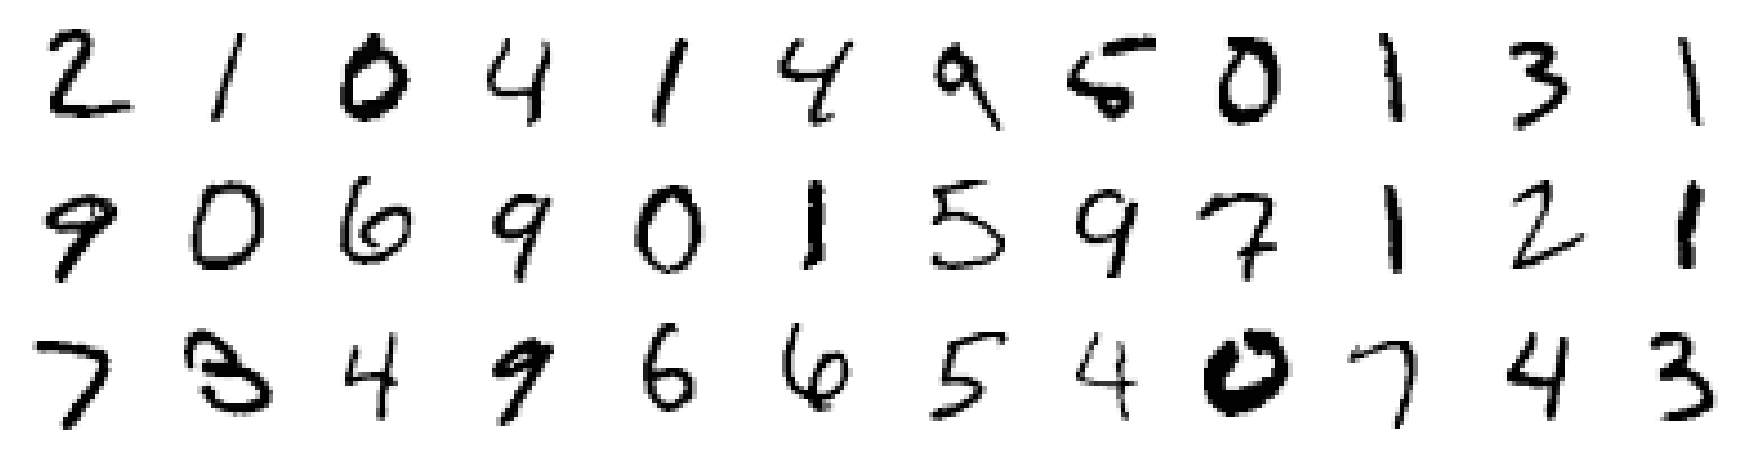
\includegraphics[width=0.9\textwidth]{img/tf/mnist.png}
\end{tabular}
\end{figure}
\end{frame}


\begin{frame}[fragile]{MNIST Dataset}
Due to its simplicity (in 2017!) the MNIST dataset is often considered to be the "Hello World!" in the Machine Learning framework.\\
\vspace{0.5cm}
In \texttt{lab\_utils.py} I already implemented a function \texttt{get\_mnist\_data} that handles the download and loading of the dataset.\\
\begin{verbatim}
    # Load MNIST data
    mnist = get_mnist_data('/tmp/mnist', verbose=True)
\end{verbatim}
\end{frame}


%%%%%%%%%%%%%%%%%%%%%%%%%%%%%%%%%%%%%%%%%%%%%%%%%%%%%%%%%%%%%%%%%%
%%%%%%%%%%%%%%%%%%%%%%%%%%%%%%%%%%%%%%%%%%%%%%%%%%%%%%%%%%%%%%%%%%
%%%%%%%%%%%%%%%%%%%%%%%%%%%%%%%%%%%%%%%%%%%%%%%%%%%%%%%%%%%%%%%%%%

\section{MNIST Classification}

%%%%%%%%%%%%%%%%%%%%%%%%%%%%%%%%%%%%%%%%%%%%%%%%%%%%%%%%%%%%%%%%%%

\begin{frame}{Goal}
The \textbf{goal} of this practice is to \textbf{implement a convolutional neural network to perform 10-class classification} on the MNIST dataset.
\end{frame}

%%%%%%%%%%%%%%%%%%%%%%%%%%%%%%%%%%%%%%%%%%%%%%%%%%%%%%%%%%%%%%%%%%

\begin{frame}{Outline}
Suggested way to proceed:
\begin{itemize}
\item In the previous practice we implemented a fully-connected net to solve the very same task. Start from your previous working example and change the model to a convolutional net.
\end{itemize}
\end{frame}

%%%%%%%%%%%%%%%%%%%%%%%%%%%%%%%%%%%%%%%%%%%%%%%%%%%%%%%%%%%%%%%%%%

\begin{frame}{Useful Functions}
To this purpose, you may find useful the following functions:
\begin{itemize}
\item \texttt{tf.reshape}
\item \texttt{tf.layers.conv2d}
\item \texttt{tf.layers.max\_pooling2d}
\item \texttt{tf.nn.dropout}
\item \texttt{tf.layers.dense}
\end{itemize}
Please refer to the docs to know the exact API.
\end{frame}

%%%%%%%%%%%%%%%%%%%%%%%%%%%%%%%%%%%%%%%%%%%%%%%%%%%%%%%%%%%%%%%%%%
%%%%%%%%%%%%%%%%%%%%%%%%%%%%%%%%%%%%%%%%%%%%%%%%%%%%%%%%%%%%%%%%%%
%%%%%%%%%%%%%%%%%%%%%%%%%%%%%%%%%%%%%%%%%%%%%%%%%%%%%%%%%%%%%%%%%%

\section{Tiles Segmentation}

\begin{frame}{Tiles Dataset}
In order to get your hands dirty with a fully convolutional architecture, I prepared a toy dataset that you can use to tackle the task of segmentation.\\
\vspace{0.5cm}
The \textbf{Tiles Dataset} consists of 64x64 images in which a 20x20 square has been drawn in a random location. Both the background and the foreground color have been chosen randomly for each image. Eventually, gaussian noise has been added to both.\\
\vspace{0.5cm}
The dataset is composed of 10000 training examples, 1000 validation examples and 1000 test examples.
\end{frame}

%%%%%%%%%%%%%%%%%%%%%%%%%%%%%%%%%%%%%%%%%%%%%%%%%%%%%%%%%%%%%%%%%%

\begin{frame}{Tiles Dataset}
The goal is to segment the square in each image. This is a \textbf{toy example of binary segmentation} (e.g. \textit{foreground} vs \textit{background}).\\
\vspace{0.5cm}
\textbf{For this task, the output of the network must be itself an image.}
\begin{figure}
\begin{tabular}{c}
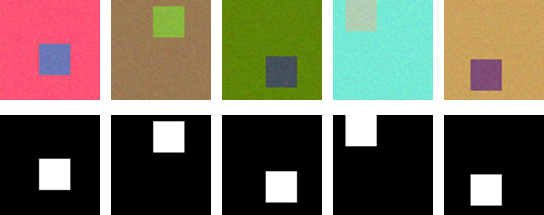
\includegraphics[width=0.75\textwidth]{img/tf/tiles_dataset.png}
\end{tabular}
\end{figure}
\end{frame}

%%%%%%%%%%%%%%%%%%%%%%%%%%%%%%%%%%%%%%%%%%%%%%%%%%%%%%%%%%%%%%%%%%

\begin{frame}{Useful Functions}
Besides all functions previously introduced, these functions might also be useful:
\begin{itemize}
\item \texttt{tf.image.resize\_bilinear}
\item \texttt{tf.transpose}
\item \texttt{tf.gather}
\item \texttt{tf.expand\_dims}
\item \texttt{tf.nn.softmax\_cross\_entropy\_with\_logits}
\end{itemize}
Please refer to the docs to know the exact API.
\end{frame}

%%%%%%%%%%%%%%%%%%%%%%%%%%%%%%%%%%%%%%%%%%%%%%%%%%%%%%%%%%%%%%%%%%

\begin{frame}[fragile]{Loading the Data}
Minimal working example for loading the data:
\begin{verbatim}
from lab_utils import load_tiles_dataset_from_cache
from lab_utils import TilesDataset

if __name__ == '__main__':
    cache_path = 'data/tiles_dataset.pickle'
    tiles_data = load_tiles_dataset_from_cache(cache_path)
\end{verbatim}
\end{frame}

%%%%%%%%%%%%%%%%%%%%%%%%%%%%%%%%%%%%%%%%%%%%%%%%%%%%%%%%%%%%%%%%%%

\begin{frame}{Outline}
\begin{itemize}
\item Load the tiles data and take your time to explore the dataset structure
\item Keep in mind that to use categorical \textit{cross-entropy} you have to convert the targets into one-hot encoding. If you instead feel quick-and-dirty, you might try to use \textit{MSE} loss and see what happens.
\item Visualizing the output of the model in TensorBoard is a good way to get a feeling of what the model is doing. To this purpose \texttt{tf.summary.image} could be useful.
\end{itemize}
\end{frame}

%%%%%%%%%%%%%%%%%%%%%%%%%%%%%%%%%%%%%%%%%%%%%%%%%%%%%%%%%%%%%%%%%%

\begin{frame}{TensorBoard Reminder}
\textbf{TensorBoard} is a suite of visualization tools integrated with TensorFlow. You can use TensorBoard to visualize your TensorFlow graph, plot quantitative metrics about the execution of your graph, and show additional data like images that pass through it.
\begin{figure}
\begin{tabular}{c}
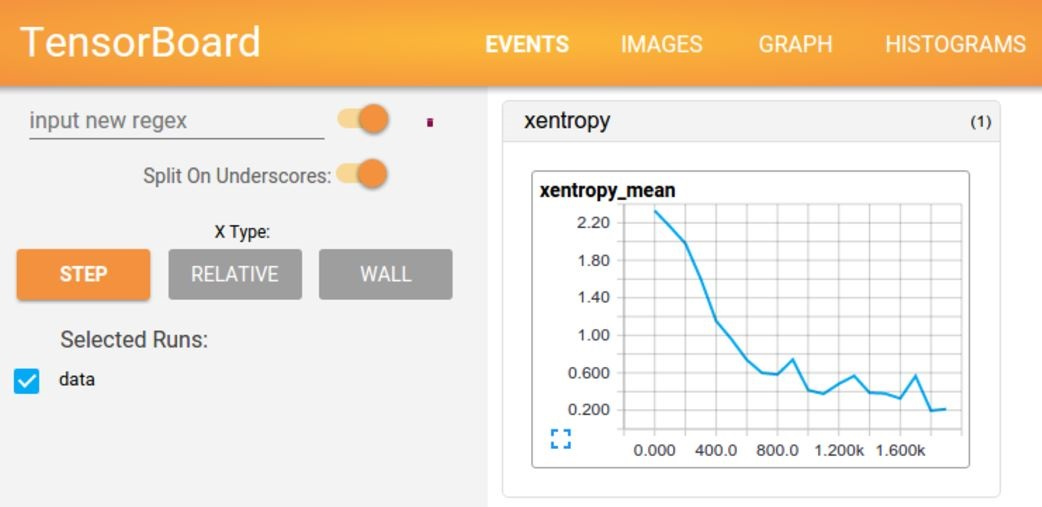
\includegraphics[width=0.7\textwidth]{img/tf/tensorboard.jpg}
\end{tabular}
\end{figure}
\end{frame}

%%%%%%%%%%%%%%%%%%%%%%%%%%%%%%%%%%%%%%%%%%%%%%%%%%%%%%%%%%%%%%%%%%

\begin{frame}{TensorBoard Reminder}
From a very high-level perspective, the lifecycle is the following:
\begin{itemize}
\item \textbf{tf.summary} operations can be attached to the nodes you'd like to collect summary data from.
\item \textbf{tf.summary.FileWriter} object is in charge of writing generated logs to a certain directory \texttt{logdir}
\item \textbf{TensorBoard} can be launched from command line as\\
\texttt{tensorboard --logdir=<logdir>}. TensorBoard is now available through your web browser at \texttt{localhost:6006}.
\end{itemize}
Official tutorial here: \url{https://www.tensorflow.org/get_started/summaries_and_tensorboard}
\end{frame}

\begin{frame}{TensorBoard Reminder}
This is an example of what you may see while training:
\begin{figure}
\centering
\begin{tabular}{c}
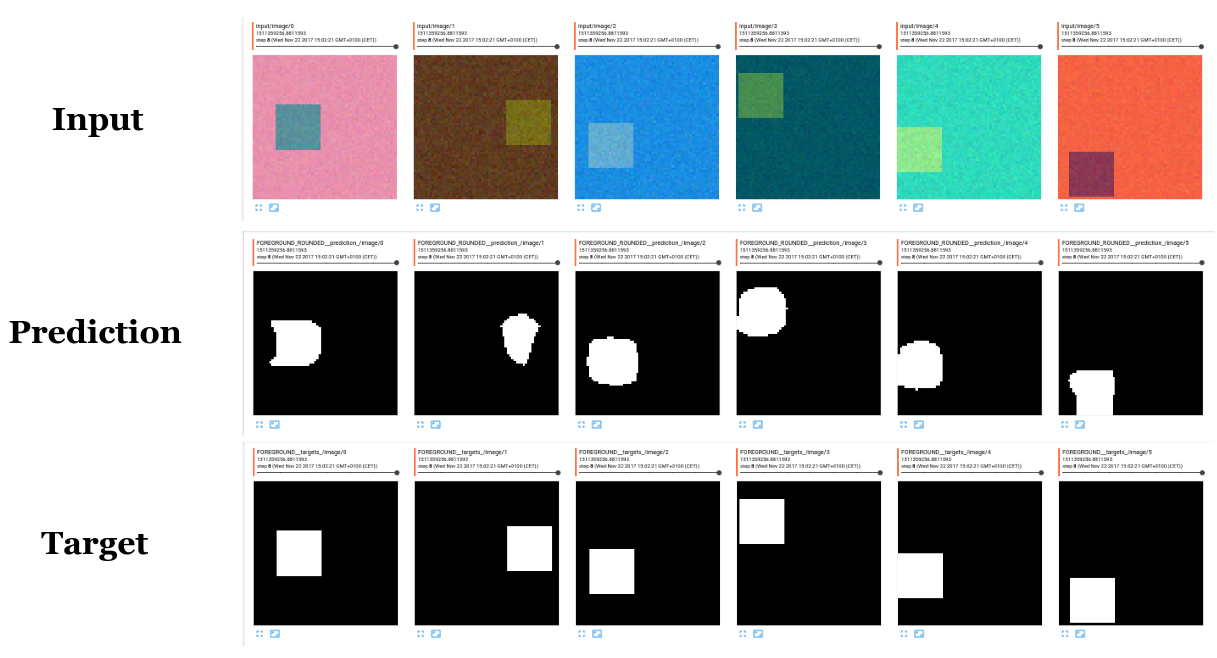
\includegraphics[width=0.8\textwidth]{img/tf/tensorboard_tiles.png}
\end{tabular}
\end{figure}
\end{frame}

%%%%%%%%%%%%%%%%%%%%%%%%%%%%%%%%%%%%%%%%%%%%%%%%%%%%%%%%%%%%%%%%%%

\begin{frame}{Tiles Dataset}
\centering{
\Large{Good Luck!}
}
\end{frame}

%%%%%%%%%%%%%%%%%%%%%%%%%%%%%%%%%%%%%%%%%%%%%%%%%%%%%%%%%%%%%%%%%%

%%%%%%%%%%%%%%%%%%%%%%%%%%%%%%%%%%%%%%%%%%%%%%%%%%%%%%%%%%%%%%%%%%
%%%%%%%%%%%%%%%%%%%%%%%%%%%%%%%%%%%%%%%%%%%%%%%%%%%%%%%%%%%%%%%%%%
%%%%%%%%%%%%%%%%%%%%%%%%%%%%%%%%%%%%%%%%%%%%%%%%%%%%%%%%%%%%%%%%%%

\section{References}

\begin{frame}[t, allowframebreaks]
\frametitle{References}
\bibliographystyle{abbrv}
\bibliography{bibliography}
\end{frame}

\end{document}